\section{Bewertung verschiedener DFT-Größen}\label{sec:AnalyseBewertungTwiddlefaktornMatrizen}

In diesem Abschnitt werden verschiedene Größen von Twiddlefaktor-Matrizen auf ihre Werte untersucht und bewertet.
Ziel ist es aus den in Frage kommenden jene zu ermitteln, die die trivialsten Berechnungen bei einer 
Multiplikation erfordert. Von Interesse sind aufgrund des dualen Zahlensystems Matrizen mit Werten, die sich einerseits 
mit wenigen Bits darstellen lassen und andererseits nur Bit-shifting zur Folge haben. Beide Anforderungen bedingen 
sich in der Regel gegenseitig.

In der folgenden Tabelle \ref{tab:DFT-TwiddlefaktorMatrizenBewertung} werden die 8$\times$8, 9$\times$9, 12$\times$12, 15$\times$15 sowie 16$\times$16-Matrix einander gegenüber gestellt.
Da die Sensormatrix aus 8$\times$8 Sensoren aufgebaut ist, besteht ein Interesse an einer ungeraden Matrix. Dies hätte den Vorteil, dass
sich über dem Mittelpunkt der Sensormatrix kein Element der Twiddlefaktormatrix befindet. Auf diese Weise ließe sich die ... einfacher ermitteln.
Bekannt ist jedoch auch,
dass die \gls{fft} auf Matrizen mit den Abmessungen 2$^n$ basiert und es sich hierbei um ein sehr schnelles und effizientes Verfahren handelt. 
Deshalb werden auch Matrizen mit gerader Anzahl an Elementen untersucht.
Die Beurteilung basiert auf dem Octave-Skript \ref{src:dft_bewertung}


 \vspace{1cm}
 \begingroup
  \renewcommand*{\arraystretch}{1.2} % Zeilenabstand der Tabelle
  \begin{table}[!ht]
  \centering
  \caption{Bewertung der DFT-Twiddlefaktor-Matrizen}
   \begin{tabular}{lccccc}
   \hline
    N							& 8	& 9	& 12	& 15		& 16 \\
    \hline
    N$\times$N						& 64	& 81	& 144	& 225		& 256 \\
    \rowcolor{lightgray}
    trivial $\Re$ 					& 48	& 45	& 128	& 81		& 128 \\
    \rowcolor{lightgray}
    nicht triv. $\Re$					& 16	& 36	& 16	& 144		& 128 \\
    triv. $\Im$ 					& 48	& 21	& 96	& 45		& 128 \\
    nicht triv. $\Im$ 					& 16	& 60	& 48	& 180		& 128 \\
    \rowcolor{lightgray}
    $\sum$ triv. 					& 96	& 66	& 224	& 126		& 256 \\
    \rowcolor{lightgray}
    $\sum$ nicht triv. 					& 32	& 96	& 64	& 324		& 256 \\
    Anzahl verschiedener nicht trivialer Werte          & 1     & 7     & 1     & 13            & 3 \\
    Verhältnis  $\sum$ trivial / $\sum$ nicht trivial	& 3	& 0,6875& 3,5	& 0,3889	& 1\\
    \hline
   \end{tabular}
   \label{tab:DFT-TwiddlefaktorMatrizenBewertung}
  \end{table}
 \endgroup
 \vspace{1cm}
 
 
%   \vspace{1cm}
%  \begingroup
%   \renewcommand*{\arraystretch}{1.2} % Zeilenabstand der Tabelle
%   \begin{table}[!ht]
%   \centering
%   \caption{Bewertung der DFT-Twiddlefaktor-Matrizen}
%    \begin{tabular}{lccccc}
%    \hline
%     N					& 8	& 9	& 12	& 15		& 16 \\
%     \hline
%     \rowcolor{lightgray}
%     N$\times$N				& 64	& 81	& 144	& 225		& 256 \\
%     trivial $\Re$ 			& 48	& 45	& 128	& 81		& 128 \\
%     nicht triv. $\Re$			& 16	& 36	& 16	& 144		& 128 \\
%     \rowcolor{lightgray}
%     triv. $\Im$ 			& 48	& 21	& 96	& 45		& 128 \\
%     \rowcolor{lightgray}
%     nicht triv. $\Im$ 			& 16	& 60	& 48	& 180		& 128 \\
%     $\sum$ triv. 			& 96	& 66	& 224	& 126		& 256 \\
%     $\sum$ nicht triv. 			& 32	& 96	& 64	& 324		& 256 \\
%     \rowcolor{lightgray}
%     Verhältnis 				& 3*	& 0,6875& 3,5	& 0,3889	& 1\\
%     \hline
%    \end{tabular}
%    \label{tab:DFT-TwiddlefaktorMatrizenBewertung}
%   \end{table}
%  \endgroup
%  \vspace{1cm}
%  
 
 
 Als triviale Werte werden 0, $\pm$0,5 sowie $\pm$1 aufgefasst.
 Andere Werte die sich gut binär darstellen lassen
 tauchen nicht auf. Alle übrigen Werte werden als nicht trivial betrachtet, da eine Multiplikation mit ihnen
 eine komplexere Berechnung bedeutet.
 
 Bei der 8$\times$8 Matrix gibt es, wie in Grafik \ref{pic:Einheitskreis_Faktoren} zu sehen, als nicht trivialen Wert mit $\abs{\nicefrac{\sqrt{2}}{2}}$ für Real- und 
 Imaginärteil nur einen einzigen Wert, welche dazu noch gemeinsam auftreten. Dies liegt daran, dass
 der Einheitskreis geachtelt wird und für beispielsweise $\frac{2\cdot\pi}{8}=\frac{\pi}{4}$ Sinus und Cosinus identisch sind. Darüberhinaus ist dies auch 
 der einzige Wert, der sowohl einen Real- aus auch einen Imaginärteil besitzt. Alle anderen Faktoren haben in einem von beiden Teilen $\abs{1}$ und somit im anderen Teil 0.
 
 In der bereits erwähnten Grafik \ref{pic:Einheitskreis_Faktoren} sind zur Veranschaulichung alle möglichen Zeiger der Twiddlefaktoren ($W_{m,n}$) für die 8$\times$8 Matrix dargestellt. 
 Berechnet werden diese mit der
 Gleichung (\ref{eq:Twiddlefaktorenberechnung}), wobei es sich bei $N$ um die Anzahl der Elemente im Vektor bzw. der Spalte einer Matrix von Werten im Zeitbereich 
 handelt. $n$ ist der Laufindex über die einzelnen Elemente, $m$ das Äquivalent für den zu berechnenden Vektor (Matrixspalte) im Frequenzbereich. Beide 
 fangen bei 0 an und laufen entsprechend bis $N-1$.


 
 
 Hieraus resultiert, dass die Hälfte der Berechnungen der nicht trivialen Werte, die für die reelle Matrix gemacht werden müssen,
 direkt für den imaginären Anteil übernommen werden können. Die andere Hälfte muss über die Bildung des 2er-Komplements lediglich negiert werden, was ein 
 bedeutend geringerer Aufwand ist, als eine Multiplikation. 
 Deshlab ist das berechnete Verhältnis von 3 in Tabelle \ref{tab:DFT-TwiddlefaktorMatrizenBewertung} in Wirklichkeit deutlich höher und übertrifft mit 7 die 12$\times$12
 Matrix um den Faktor 2. Dies gilt unter der Annahme, dass die Bildung des 2er-Komplements nicht berücksichtigt wird, was zumindest einer besseren Näherung 
 entspricht, als es als eine volle Multiplikation zu werten.
 
 Hierzu Abschnitt Abschätzung des Rechenaufwandes?
 
 Anfangs wurde angenommen, dass das 1er-Komplement eine gute Wahl sein könnte, da hierbei die Darstellung negativer Zahlen einzig durch Setzen des vordersten 
 Bit (\gls{msb}) erfolgt. Auf diese Weise könnte immer das selbe Resultat für den Imaginär- wie für den Realteil verwendet werden, das Vorzeichen würde sich über eine 
 einfache XOR-Verknüpfung beider \gls{msb} ergeben.
 Diesem Vorteil steht jedoch eine komlexere Subtraktion (bzw. Addition negativer Zahlen) gegenüber. Der zusätzliche Aufwand entspricht 
 relativ genau dem der Bildung des 2er-Komplements. Aus diesem Grund wurde sich für dieses entschieden, da es deutlich gängiger ist und weitere Vorteile bringt wie 
 beispielsweise keine Doppeldeutigkeit durch eine negative Null hat.
 
 In Abbildung (\ref{pic:Twiddlefaktoren_Darstellung8x8}) sind zur weiteren Veranschaulichung die komplexen Zeiger der Twiddlefaktoren dargestellt. Sie sind aufgeteilt auf 8 
 Einheitskreise, wobei jeder einen Laufindex (m) des Zeitbereichs abdeckt. In den einzelnen Kreisen sind wiederum alle Laufindexe (n) des Frequenzbereichs zu sehen.
 
 Anhand der Gleichung ((\ref{eq:Twiddlefaktorenberechnung})) für die Twiddlefaktoren und des Einheitskreises in Abb (\ref{pic:Einheitskreis_Faktoren}) lässt sich erkennen, 
 dass die Zeiger im Gegenuhrzeigersinn rotieren und sich sowohl für den Realteil als auch den Imaginärteil gleichmäßig auf positive und negative
 Werte aufteilen. Das lässt sich ausnutzen, um keine Negationen der Eingangs- / Zwischenwerte erfolgen muss. Darüber hinaus
 minimiert sich bei geschickter Anordnung das Risiko eines Überlaus. Da zur Sicherheit dennoch nach jeder Addition / Subtraktion
 das Ergebnis durch einen Bitshift halbiert wird. Da über die Eingangswerte die Annahme getroffen werden kann, dass 
 aufeinanderfolgende Werte das selbe Vorzeichen haben, kann hier noch weiter die Genauigkeit optimiert werden. 


 \begin{figure}[!t]
  \centering
  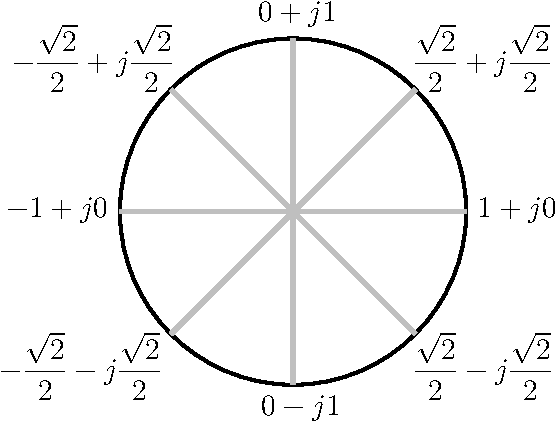
\includegraphics[width=0.3\textwidth]{img/Einheitskreis-crop.pdf}
  \captionof{figure}{Einheitskreis mit relevanten Werten}
  \label{pic:Einheitskreis_Faktoren}
\end{figure}
  
 


\begin{figure}[!ht]
 \centering
 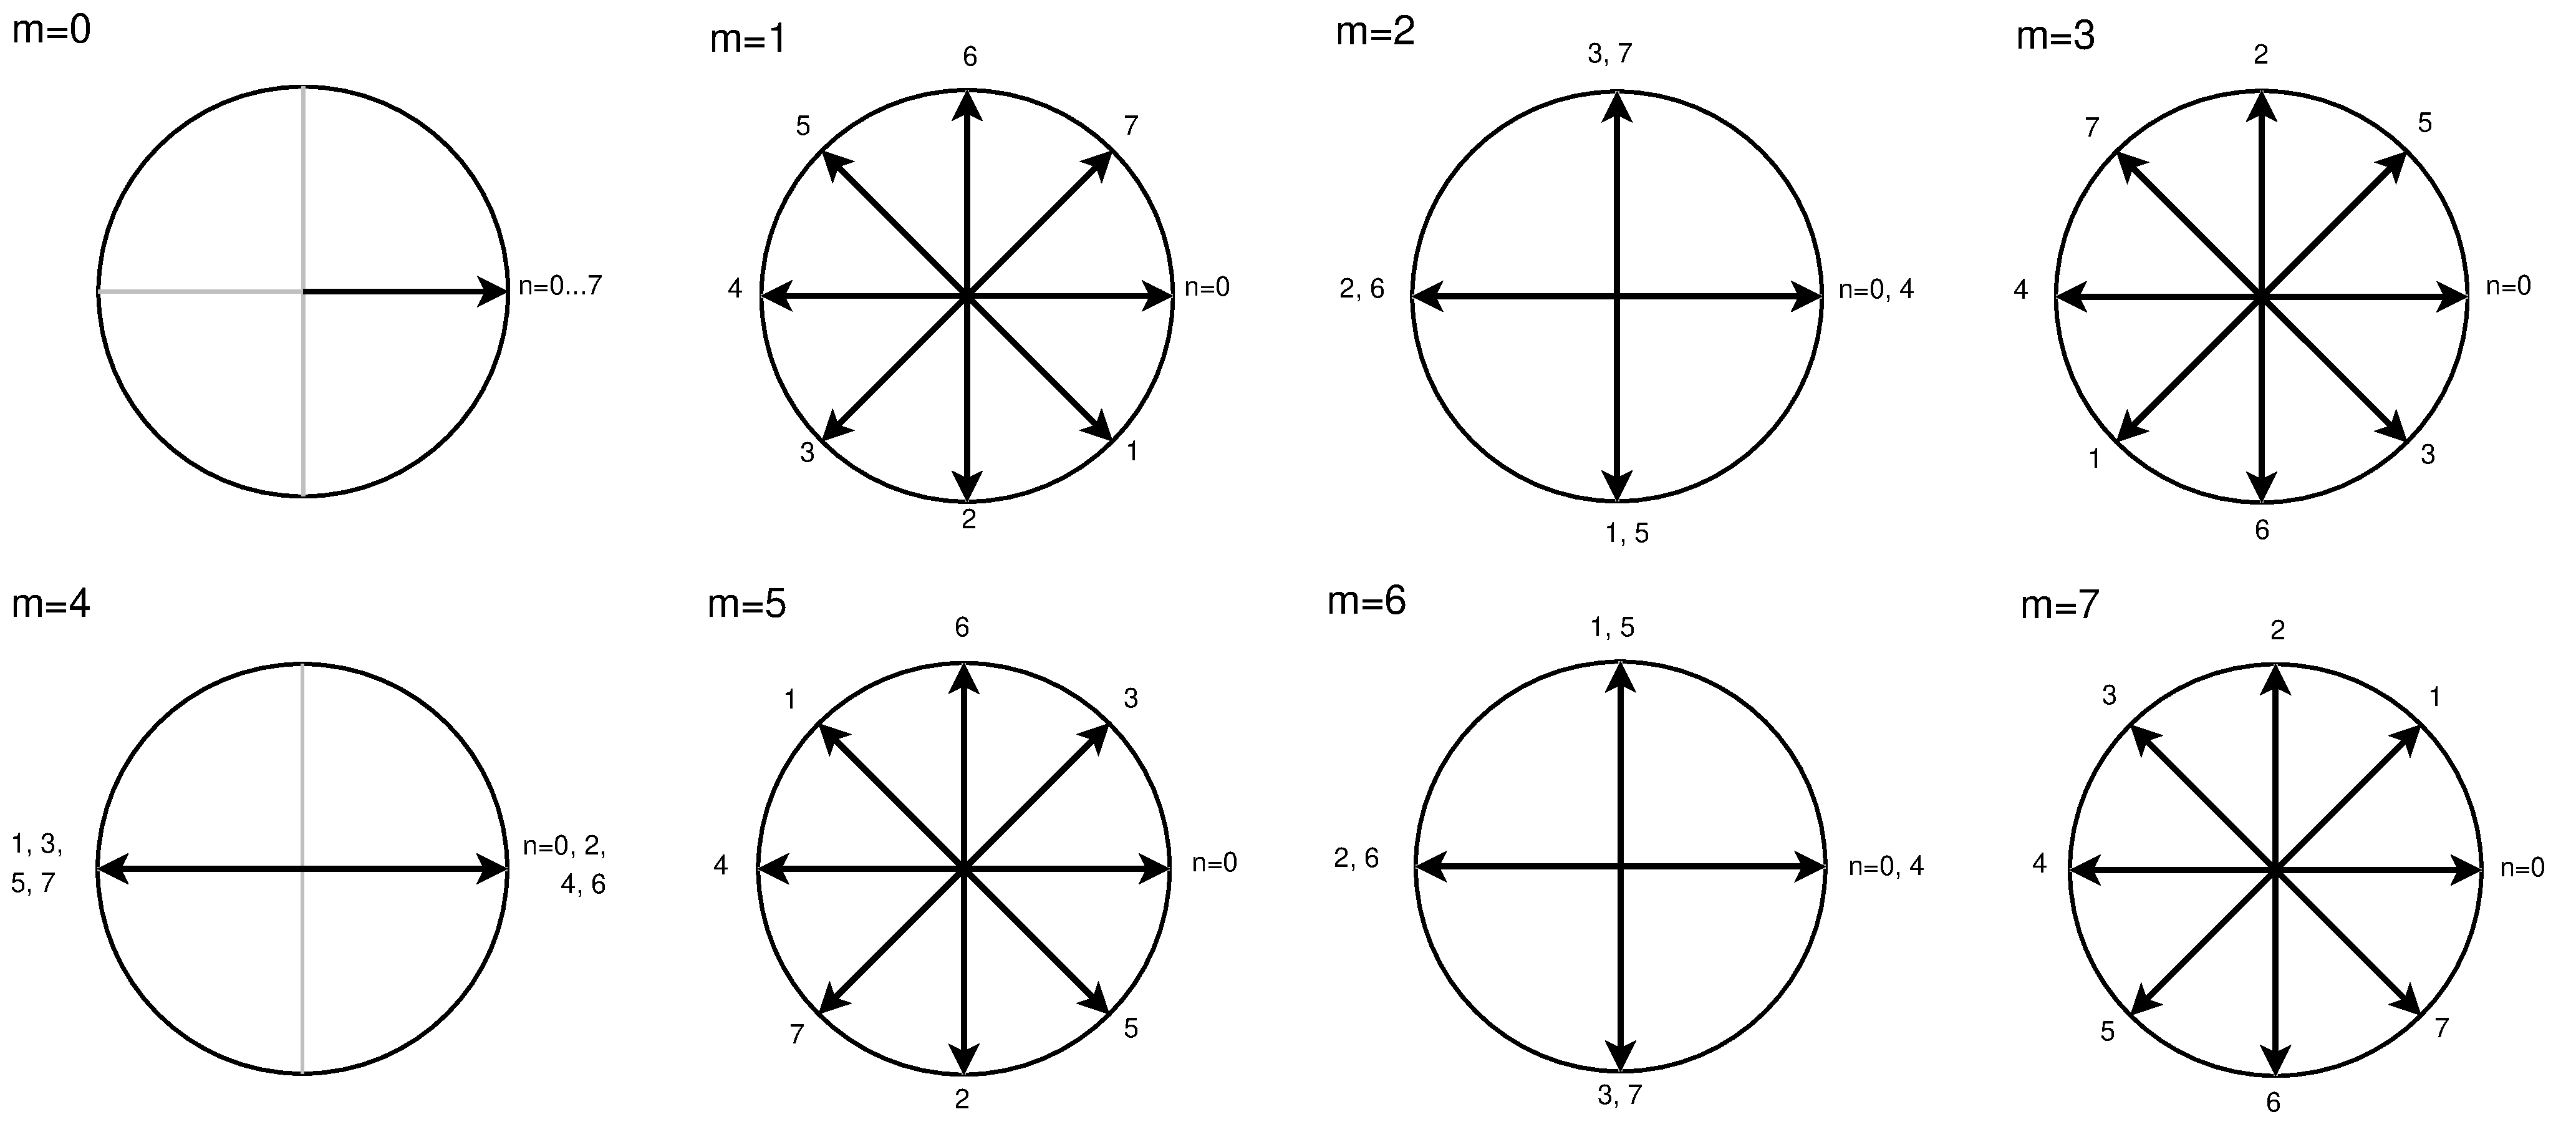
\includegraphics[width=0.9\textwidth]{img/Twiddlefaktoren_Einheitskreis.eps}
 \caption{Twiddlefaktoren der 8$\times$8-Matrix, aufgeteilt auf die Laufindexe}
 \label{pic:Twiddlefaktoren_Darstellung8x8}
\end{figure}

\vspace{0.5cm}


 

\begin{minipage}{0.9\textwidth}
\begingroup
 \renewcommand*{\arraystretch}{0.95} % Zeilenabstand der Tabelle

\begin{center}
  \[
   \stackrel{\mbox{$Re\{W\}$}}{
    \begin{bmatrix}
     \myboxOnePos 	& \myboxOnePos 		& \myboxOnePos 	& \myboxOnePos 		& \myboxOnePos 	& \myboxOnePos 		& \myboxOnePos 	& \myboxOnePos \\
     \myboxOnePos 	& \myboxSqrtPos 	& \myboxZero 	& \myboxSqrtNeg		& \myboxOneNeg	& \myboxSqrtNeg		& \myboxZero	& \myboxSqrtPos \\
     \myboxOnePos 	& \myboxZero 		& \myboxOneNeg 	& \myboxZero 		& \myboxOnePos 	& \myboxZero 		& \myboxOneNeg 	& \myboxZero \\
     \myboxOnePos 	& \myboxSqrtNeg 	& \myboxZero 	& \myboxSqrtPos 	& \myboxOneNeg 	& \myboxSqrtPos 	& \myboxZero 	& \myboxSqrtNeg \\
     \myboxOnePos 	& \myboxOneNeg 		& \myboxOnePos 	& \myboxOneNeg 		& \myboxOnePos 	& \myboxOneNeg 		& \myboxOnePos 	& \myboxOneNeg \\
     \myboxOnePos 	& \myboxSqrtNeg 	& \myboxZero 	& \myboxSqrtPos 	& \myboxOneNeg 	& \myboxSqrtPos 	& \myboxZero 	& \myboxSqrtNeg \\
     \myboxOnePos 	& \myboxZero 		& \myboxOneNeg 	& \myboxZero 		& \myboxOnePos 	& \myboxZero 		& \myboxOneNeg 	& \myboxZero \\
     \myboxOnePos 	& \myboxSqrtPos 	& \myboxZero 	& \myboxSqrtNeg		& \myboxOneNeg	& \myboxSqrtNeg		& \myboxZero	& \myboxSqrtPos 
    \end{bmatrix}
   }
   \hspace{1cm}
   \stackrel{\mbox{$Im\{W\}$}}{
    \begin{bmatrix}
     \myboxZero 	& \myboxZero 		& \myboxZero 	& \myboxZero 		& \myboxZero 	& \myboxZero 		& \myboxZero 	& \myboxZero \\
     \myboxZero 	& \myboxSqrtNeg 	& \myboxOneNeg 	& \myboxSqrtNeg		& \myboxZero	& \myboxSqrtPos		& \myboxOnePos	& \myboxSqrtPos \\
     \myboxZero 	& \myboxOneNeg 		& \myboxZero 	& \myboxOnePos 		& \myboxZero 	& \myboxOneNeg 		& \myboxZero 	& \myboxOnePos \\
     \myboxZero 	& \myboxSqrtNeg 	& \myboxOnePos 	& \myboxSqrtNeg 	& \myboxZero 	& \myboxSqrtPos 	& \myboxOneNeg 	& \myboxSqrtPos \\
     \myboxZero 	& \myboxZero 		& \myboxZero 	& \myboxZero 		& \myboxZero 	& \myboxZero 		& \myboxZero 	& \myboxZero \\
     \myboxZero 	& \myboxSqrtPos 	& \myboxOneNeg 	& \myboxSqrtPos		& \myboxZero 	& \myboxSqrtNeg 	& \myboxOnePos 	& \myboxSqrtNeg \\
     \myboxZero 	& \myboxOnePos 		& \myboxZero 	& \myboxOneNeg 		& \myboxZero 	& \myboxOnePos 		& \myboxZero 	& \myboxOneNeg \\
     \myboxZero 	& \myboxSqrtPos 	& \myboxOnePos 	& \myboxSqrtPos		& \myboxZero	& \myboxSqrtNeg		& \myboxOneNeg	& \myboxSqrtNeg 
    \end{bmatrix}
   }
  \]
  \captionof{figure}{Matrizen-Darstellung der Twiddlefaktoren aufgeteilt nach \\Real- und Imaginärteil}
  \label{pic:MatrizenDarstellungTwiddlefaktoren}
 
\vspace{0.5cm}
  Legende: $\myboxOnePos$ = 1 \quad $\myboxOneNeg$ = -1 \quad $\myboxZero$ = 0 \quad $\myboxSqrtPos$ = $\nicefrac{\sqrt{2}}{2}$ \quad $\myboxSqrtNeg$ = -$\nicefrac{\sqrt{2}}{2}$
\end{center}
\endgroup
\end{minipage}


\vspace{0.5cm}


Sowohl der Abbildung \ref{pic:Twiddlefaktoren_Darstellung8x8} als auch insbesondere der Darstellung \ref{pic:MatrizenDarstellungTwiddlefaktoren} lassen sich sehr gut die 
Symmetrien erkennen, die diese Twiddlefaktormatrix so vorteilhaft machen.